\chapter{Introduction and Astrobiological Context}\label{chap:introduction}

\section{Context and Motivation: The Era of Atmospheric Characterization}\label{sec:context_motivation}

For centuries, the inquiry into whether biological life exists beyond Earth was relegated to theoretical speculation, philosophical discourse, and rudimentary statistical formulations such as the Drake Equation. Observational astronomy remained fundamentally constrained by instrument sensitivity, limiting exoplanetary research to indirect dynamical detections. Over the past three decades, however, pioneering spaceborne and ground-based observatories---most notably the Kepler Space Telescope and the Transiting Exoplanet Survey Satellite (TESS)---have confirmed the existence of over 5,500 exoplanets, demonstrating that planetary systems are ubiquitous throughout the Milky Way.

\notatfm{\textbf{Paradigm Shift:} Transitioning from geometric exoplanet detection to high-resolution transmission spectroscopy of atmospheric terminators.}
The successful commissioning and deployment of the James Webb Space Telescope (JWST), alongside the planned development of the Habitable Worlds Observatory (HWO), has precipitated a definitive transition in observational astrophysics: shifting from geometric discovery (kinematic radial velocity and transit photometry) to rigorous atmospheric characterization via transmission and emission spectroscopy \cite{madhusudhan2023}. When an exoplanet transits its host star, a fraction of the stellar photons traverses the annulus of the planetary upper atmosphere. The wavelength-dependent absorption of this starlight by atmospheric molecules imprints discrete absorption and emission bands onto the observed transit transmission spectrum. 

Deciphering these spectral fingerprints provides direct empirical access to the chemical inventory, thermal structure, and cloud microphysics of distant worlds. However, translating raw, photon-starved spectroscopic telemetry into robust astrobiological assertions represents an immense inferential challenge. Planetary atmospheres are complex, non-linear chemical reactors governed by stellar irradiation, atmospheric dynamics, vertical mixing, and disequilibrium photochemistry. Consequently, establishing whether an observed atmospheric composition indicates a living biosphere, an industrial technosphere, or a benign abiotic geochemical cycle requires high-dimensional probabilistic reasoning capable of simultaneously evaluating dozens of interdependent physical parameters.

\section{Scientific Motivation: Biosignatures and Technosignatures Under Causal Ambiguity}\label{sec:biosignatures_technosignatures}

The operational search for extraterrestrial life is structured around two distinct taxonomic classes of observational phenomena: biosignatures and technosignatures. 

\subsection{Atmospheric Biosignatures and the False-Positive Dilemma}
A biosignature is defined not as the direct observation of an organism, but as an atmospheric, surface, or temporal anomaly produced by biological metabolic activity that cannot be reconciled with abiotic geological, photochemical, or stellar mechanisms. The foundational paradigm for atmospheric biosignature detection rests upon the principle of extreme thermodynamic chemical disequilibrium. In a sterile planetary atmosphere, volatile gases tend toward thermodynamic equilibrium dictated by planetary bulk composition, surface temperature, pressure, and stellar ultraviolet (UV) irradiation. 

\notatfm{\textbf{Disequilibrium:} Canonical biogenic pairs (e.g., $\mathrm{O}_2$--$\mathrm{CH}_4$) maintain atmospheric steady states orders of magnitude above abiotic equilibrium.}
A pervasive global biosphere, conversely, acts as a continuous kinetic pump, injecting reduced and oxidized gases into the atmosphere at rates that vastly exceed their photochemical sink rates. The quintessential terrestrial benchmark is the simultaneous atmospheric coexistence of molecular oxygen ($\mathrm{O}_2$) and methane ($\mathrm{CH}_4$). Because $\mathrm{O}_2$ and $\mathrm{CH}_4$ photochemically react through hydroxyl radical ($\mathrm{OH}$) cascades to yield carbon dioxide ($\mathrm{CO}_2$) and water ($\mathrm{H}_2\mathrm{O}$), their steady-state coexistence at terrestrial partial pressures requires a biological replenishment flux exceeding $10^9$ molecules $\mathrm{cm}^{-2}\,\mathrm{s}^{-1}$. Absent biological methanogenesis and oxygenic photosynthesis, this chemical pair would rapidly deplete to undetectable levels on geological timescales.

However, the primary scientific obstacle in modern astrobiology is the prevalence of abiotic false positives. Non-biological mechanisms can mimic biogenic atmospheric signatures:
\begin{enumerate}
    \item \textbf{Photochemical Oxygen Accumulation:} On volatile-rich worlds orbiting active M-dwarf stars, intense extreme ultraviolet (EUV) stellar radiation drives the massive photolysis of $\mathrm{H}_2\mathrm{O}$, followed by hydrodynamic hydrogen escape to space. This process can leave behind tens of bars of abiotic residual $\mathrm{O}_2$ and ozone ($\mathrm{O}_3$), completely decoupling the presence of oxygen from biological activity.
    \item \textbf{Abiotic Methanogenesis:} Methane can be generated in substantial volumes through abiotic serpentinization and Fischer-Tropsch-type catalytic reactions in hydrothermal vents, or delivered via cometary impacts, absent any metabolic processes.
\end{enumerate}

Consequently, isolating an individual gas species in a transmission spectrum yields negligible epistemological confidence. Unambiguous biosignature attribution necessitates evaluating the entire environmental context simultaneously: stellar spectral type, chromospheric flare activity, surface gravity, planetary temperature, and the concurrent presence or absence of photochemical discriminators (such as carbon monoxide, $\mathrm{CO}$, which serves as a biological nutrient on Earth but accumulates to high concentrations in abiotic oxygen-rich scenarios).

\subsection{Technosignatures as Ultra-Rare Causal Inferences}
\notatfm{\textbf{Technosignatures:} Artificial volatile compounds (e.g., CFCs) provide unambiguous technomarkers but possess vanishingly small baseline priors ($p \ll 10^{-5}$).}
Technosignatures represent measurable evidence of technological activity, such as artificial atmospheric pollutants, orbital megastructures, or monochromatic laser emissions. Among atmospheric candidates, chlorofluorocarbons (e.g., $\text{CFC-11}$, $\text{CFC-12}$) and perfluorocarbons are particularly compelling because they possess zero known natural abiotic synthesis pathways and exhibit strong absorption bands within thermal infrared atmospheric windows. 

Nevertheless, detecting a technosignature presents a profound statistical challenge. Because technological civilizations are statistically rare or localized, the baseline prior probability of their occurrence is exceptionally low ($p \approx 10^{-5}$ to $10^{-6}$). When inferring the presence of an ultra-rare phenomenon from noisy, low-resolution astronomical data, Bayesian updating must be extraordinarily rigorous to avoid false alarms. Claiming the detection of an extraterrestrial technology requires mathematically bounded certainty that pushes classical statistical algorithms beyond their computational limits.

\subsection{The K2-18b Archetype and Epistemic Uncertainty}
\notatfm{\textbf{Target Archetype:} K2-18b exemplifies the challenge of high observational uncertainty and tentative trace species (e.g., DMS) near detection thresholds.}
This inferential complexity is epitomized by recent JWST observations of the sub-Neptune exoplanet K2-18b, situated in the habitable zone of an M2.5 dwarf star \cite{madhusudhan2023}. Spectroscopic retrieval using the NIRISS and NIRSpec instruments identified carbon-bearing molecules, specifically methane ($\mathrm{CH}_4$) and carbon dioxide ($\mathrm{CO}_2$), alongside a depleted abundance of ammonia ($\mathrm{NH}_3$). This atmospheric composition is consistent with theoretical models of a Hycean world---a planet possessing a massive liquid water ocean underlying a hydrogen-rich envelope. Notably, the retrieval models indicated tentative, low-significance evidence ($\sim 1\sigma$--$2\sigma$) of dimethyl sulfide ($\mathrm{CH}_3\mathrm{SCH}_3$, DMS), an organosulfur compound produced almost exclusively by marine phytoplankton on Earth.

\begin{figure}[htbp]
    \centering
    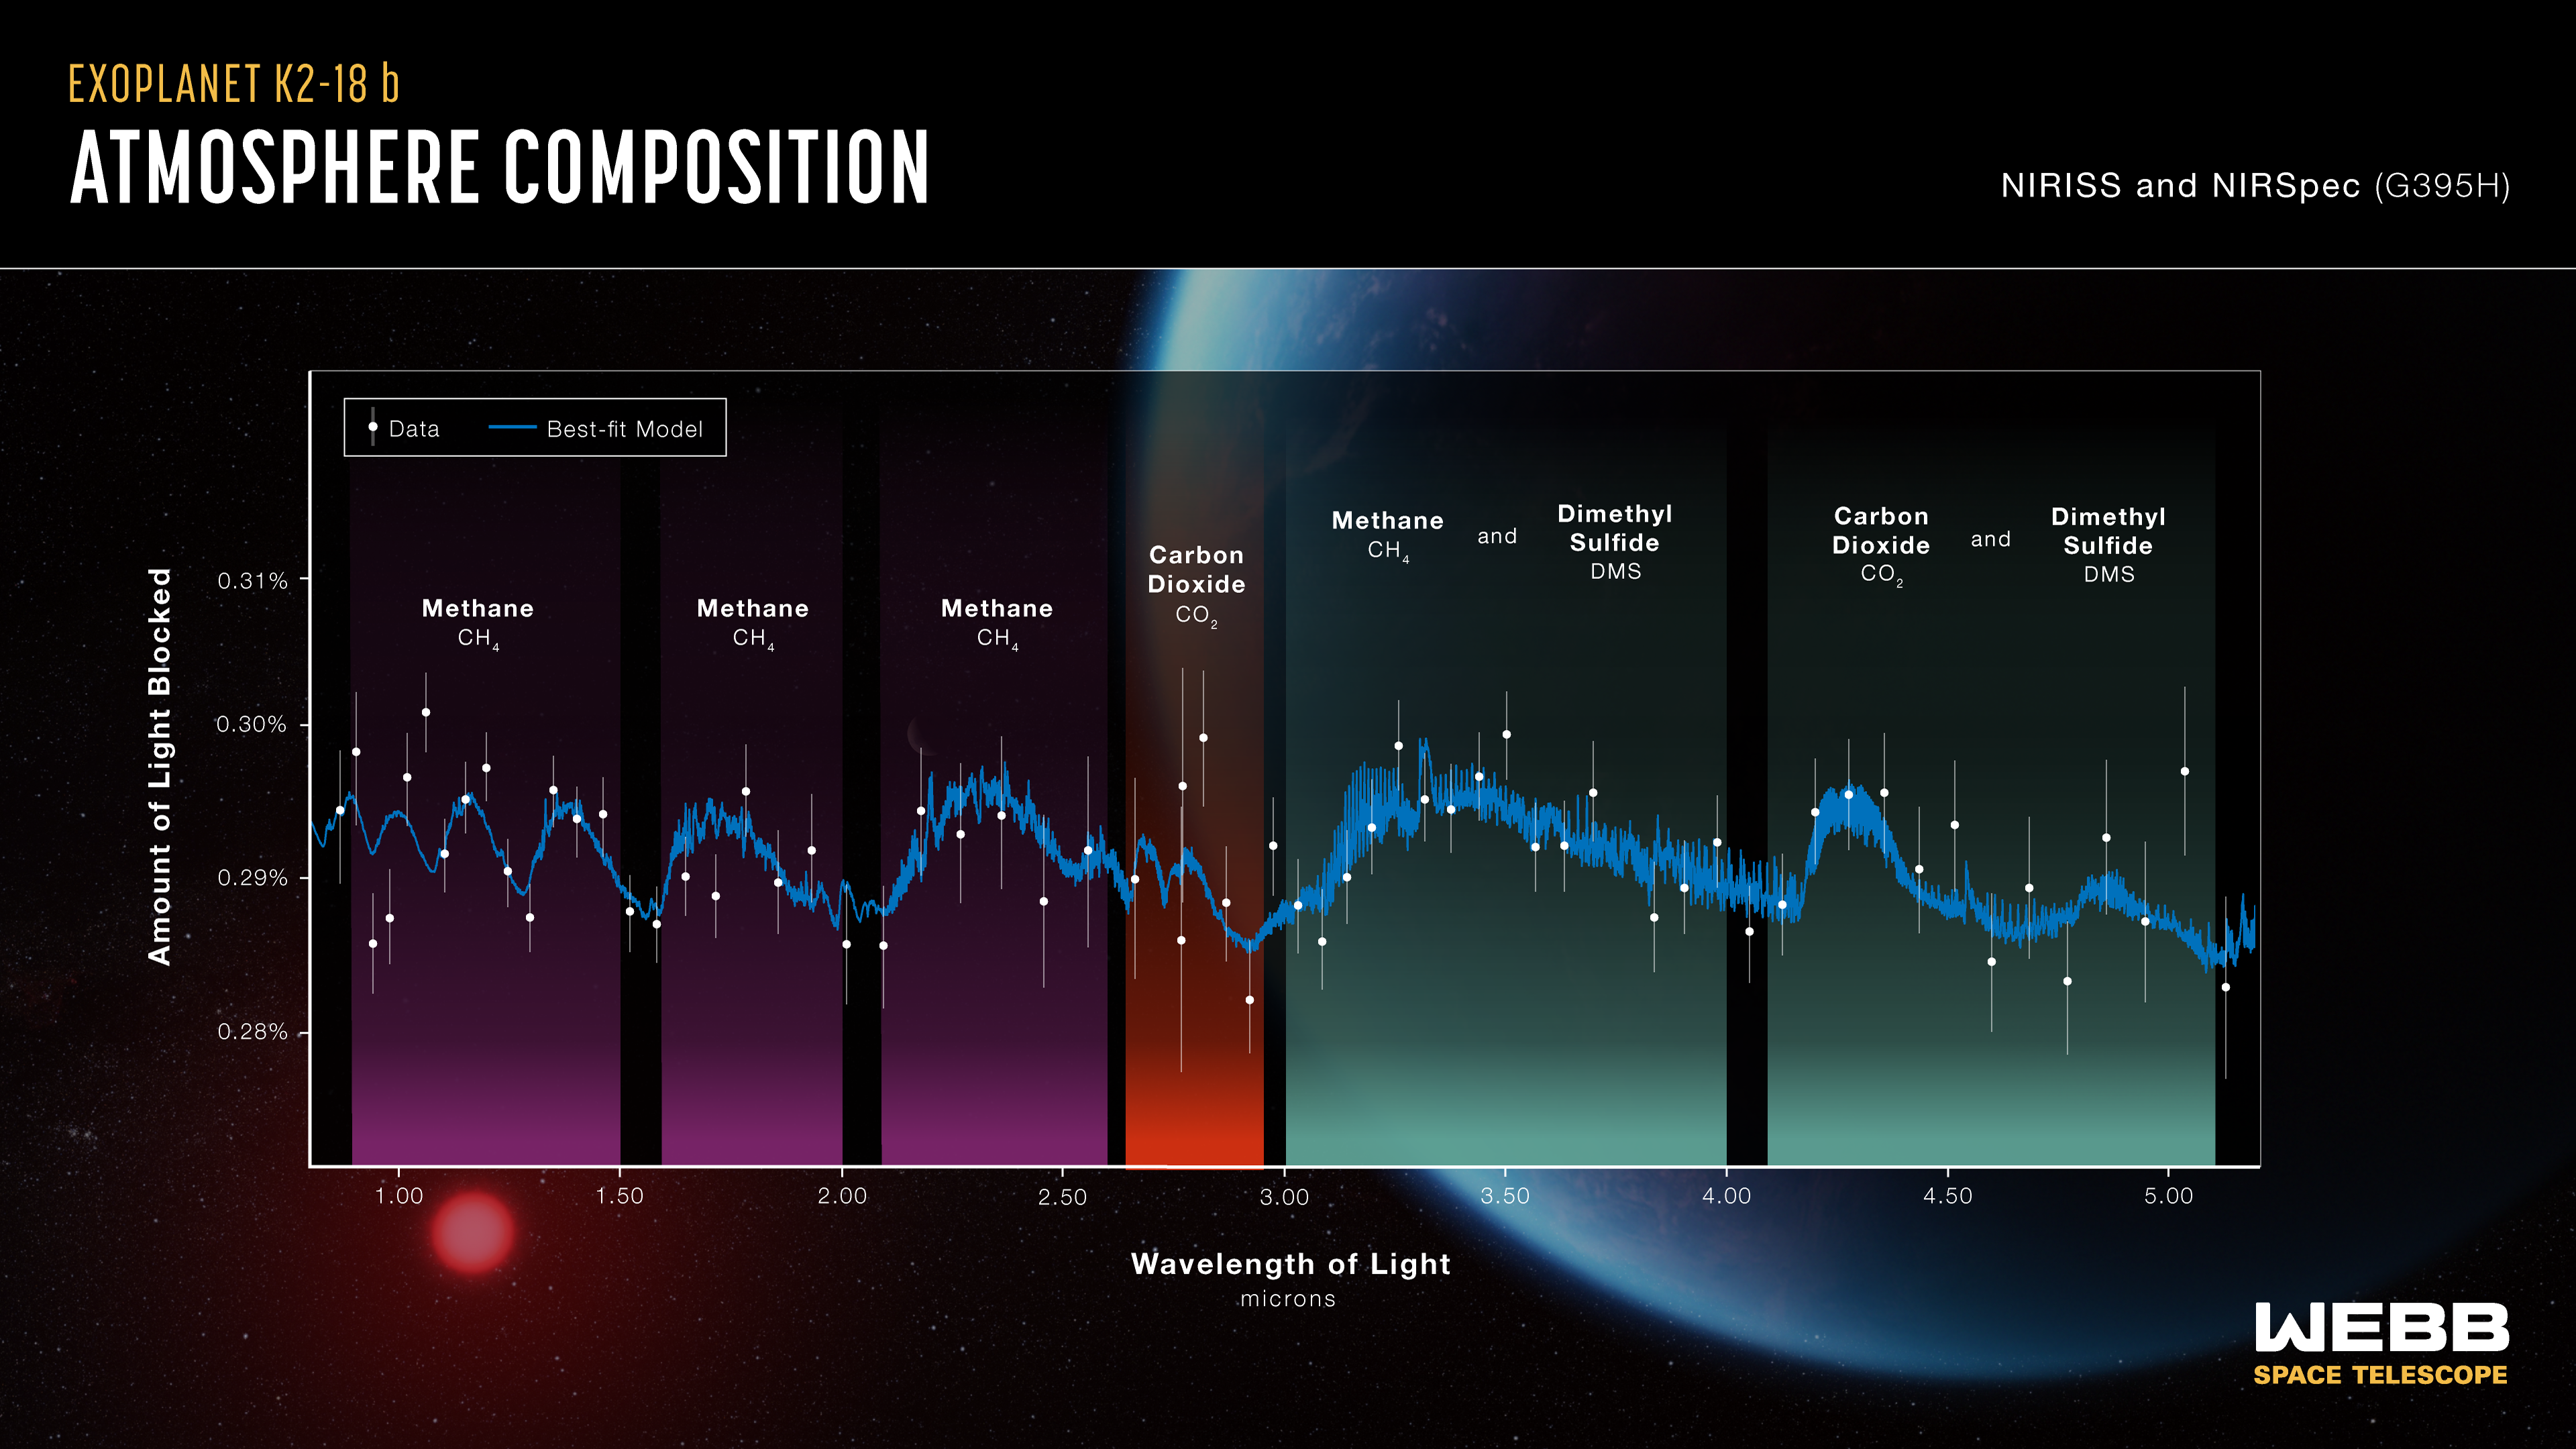
\includegraphics[width=0.95\textwidth]{figures/1.introduction/spectrum_k218b.png}
    \caption{\textbf{Transmission Spectrum of Exoplanet K2-18b (JWST NIRISS \& NIRSpec).} The observational data reveals prominent absorption features of carbon-bearing molecules ($\mathrm{CH}_4$ and $\mathrm{CO}_2$) while showing a depleted abundance of $\mathrm{H}_2\mathrm{O}$ and $\mathrm{NH}_3$. These spectral lines form the empirical baseline evidence for the astrobiological Bayesian inference model. Image credit: NASA/ESA/CSA/STScI.}
    \label{fig:k218b_spectrum}
\end{figure}

However, the astronomical community actively debates the veracity and physical interpretation of this signal. Subsequent atmospheric modeling has emphasized that the tentative $3.4\,\mu\mathrm{m}$ DMS absorption feature exhibits severe degeneracies with overlapping methane ($\mathrm{CH}_4$) and ethane ($\mathrm{C}_2\mathrm{H}_6$) opacity bands, with competing geochemical hypotheses questioning whether K2-18b harbors a habitable ocean or represents a volatile-rich, sterile mini-Neptune with a deep convective atmosphere. The observational signal-to-noise ratio is currently insufficient to rule out these photochemical degeneracies or systematic instrument artifacts. K2-18b thus represents the quintessential archetype for advanced probabilistic inference: an exoplanetary benchmark defined not by definitive biological attribution, but by coupled causal variables, degenerate geochemical and biological hypotheses, and high epistemic uncertainty near detection thresholds.

\section{Computational Problem Statement: Classical Bottlenecks in Astrobiological Inference}\label{sec:computational_problem}

To model these intricate dependencies, astrobiologists formalize planetary systems as Bayesian Networks (BNs)---Directed Acyclic Graphs (DAGs) wherein nodes represent discrete or discretized physical parameters and directed edges quantify causal or photochemical conditional dependencies \cite{pearl1988}.

\input{figures/1.introduction/figure1_dag_k218b.tex}

While Bayesian Networks offer a rigorous framework for causal reasoning, evaluating them on classical computing architectures encounters two mathematically insurmountable bottlenecks: the treewidth explosion of exact inference and the asymptotic sample variance divergence of stochastic approximation.

\subsection{The Treewidth Bottleneck in Exact Classical Inference}
Let a planetary atmosphere be modeled as a Bayesian Network $\mathcal{B} = (\mathcal{G}, \Theta)$, where $\mathcal{G} = (V, E)$ is a DAG with $N = |V|$ random variables $X = \{X_1, X_2, \dots, X_N\}$, and $\Theta$ denotes the set of Conditional Probability Tables (CPTs) parameterizing each node given its direct parents:
\begin{equation}
P(X_1, X_2, \dots, X_N) = \prod_{i=1}^N P\left(X_i \mid \mathrm{Parents}(X_i)\right).
\label{eq:bn_factorization_ch1}
\end{equation}
In astrobiological retrieval, the computational goal is to compute the posterior probability of a hidden target hypothesis (e.g., biological habitability $X_{\mathrm{bio}}$ or technosignature presence $X_{\mathrm{tech}}$) conditioned on observed spectroscopic evidence $\mathbf{E} = \mathbf{e}$:
\begin{equation}
P(X_{\mathrm{target}} \mid \mathbf{E} = \mathbf{e}) = \frac{\sum_{Y} \prod_{i=1}^N P\left(X_i \mid \mathrm{Parents}(X_i)\right)}{P(\mathbf{E} = \mathbf{e})},
\label{eq:exact_marginalization_ch1}
\end{equation}
where $Y = X \setminus \{X_{\mathrm{target}} \cup \mathbf{E}\}$ represents the set of unobserved latent environmental parameters that must be marginalized out.

\notatfm{\textbf{Exact Bottleneck:} Classical exact inference via Junction Tree is bounded by $\mathcal{O}(N \cdot d^{w+1})$, exploding exponentially as treewidth $w$ grows.}
Classical algorithms for exact inference, such as Variable Elimination (VE) and the Junction Tree Algorithm (JTA), marginalize latent variables by constructing intermediate clique potentials over triangulated chordal graphs. Cooper (1990) proved that exact inference in general Bayesian belief networks is NP-hard \cite{cooper1990}. The temporal and spatial computational complexity of the Junction Tree algorithm is strictly bounded by:
\begin{equation}
\mathcal{C}_{\mathrm{exact}} = \mathcal{O}\left(N \cdot d^{w+1}\right),
\label{eq:treewidth_bound_ch1}
\end{equation}
where $d$ is the maximum domain cardinality of the variables and $w$ is the \emph{treewidth} of the moralized, triangulated graph $\mathcal{G}$. In realistic photochemical networks, where stellar UV, redox buffers, and multi-gas feedback loops create dense cyclic dependencies, moralization introduces numerous fill-in edges. As the treewidth $w$ scales linearly with network connectivity, the required memory to store the multi-dimensional clique tensors $\tau(C_j)$ explodes exponentially, rapidly exhausting classical RAM even for moderately sized networks ($N \sim 30$--$50$).

\subsection{The Sampling Bottleneck and Rare-Event Variance Divergence}
To bypass the exponential memory wall of exact inference, classical computation relies on stochastic simulation, predominantly Markov Chain Monte Carlo (MCMC) methods such as Gibbs sampling and Metropolis-Hastings. MCMC generates empirical trajectories through the probability space, estimating posterior distributions by sample frequency counts.

However, stochastic sampling trades an intractable spatial bottleneck for a prohibitive temporal bottleneck:
\begin{enumerate}
    \item \textbf{Slow Asymptotic Convergence:} By virtue of the Central Limit Theorem, the standard error of a Monte Carlo estimator based on $M$ independent samples scales as:
    \begin{equation}
    \sigma_{\hat{p}} = \sqrt{\frac{p(1-p)}{M}} = \mathcal{O}\left(\frac{1}{\sqrt{M}}\right).
    \label{eq:mcmc_convergence_ch1}
    \end{equation}
    To gain a single additional decimal digit of inferential precision ($\epsilon \to 0.1\epsilon$), the classical simulator must increase the number of samples by a factor of 100 ($M \to 100M$).
    \item \textbf{Approximation Hardness:} Dagum and Luby (1993) demonstrated that approximating probabilistic inference in Bayesian networks within an absolute error bound $\epsilon$, or within a relative error bound $\epsilon$ for small $p$, is NP-hard \cite{dagum1993}.
    \item \textbf{Catastrophic Variance Divergence in Rare Events:} When evaluating ultra-rare target events, such as a technosignature hypothesis with baseline probability $p \ll 1$, the classical Monte Carlo estimator suffers from asymptotic instability. As formalized by L'Ecuyer et al.~(2010) \cite{lecuyer2010}, the Relative Error ($\mathrm{RE}$) of the estimator $\hat{p}$ is given by:
    \begin{equation}
    \mathrm{RE}(\hat{p}) = \frac{\sqrt{\mathrm{Var}(\hat{p})}}{p} = \frac{\sqrt{\frac{p(1-p)}{M}}}{p} = \sqrt{\frac{1-p}{M \cdot p}}.
    \label{eq:relative_error_divergence_ch1}
    \end{equation}
    As the true probability $p \to 0$, the relative variance diverges to infinity:
    \begin{equation}
    \lim_{p \to 0} \mathrm{RE}(\hat{p}) = \infty.
    \end{equation}
\end{enumerate}

\notatfm{\textbf{Rare-Event Divergence:} Relative error diverges as $\mathcal{O}(1/\sqrt{M p})$, requiring $M \ge \mathcal{O}(1/p)$ samples to resolve rare technosignatures.}
To achieve a modest relative error tolerance $\epsilon = 0.05$ on a rare technosignature with prior $p = 10^{-6}$, the classical simulator requires a prohibitive sample volume:
\begin{equation}
M \ge \frac{1-p}{\epsilon^2 \cdot p} \approx \frac{1}{(0.05)^2 \cdot 10^{-6}} = 4 \times 10^8 \text{ samples}.
\end{equation}
When embedded within iterative exoplanet atmospheric retrieval pipelines involving thousands of parameter evaluations, classical stochastic sampling becomes computationally unviable.

\section{Quantum Motivation: Foundations of Quantum Bayesian Advantage}\label{sec:quantum_motivation}

To resolve the dual bottlenecks of classical Bayesian computation, this Master's Thesis introduces a quantum computing framework combining Quantum Bayesian Networks (QBN) with Quantum Amplitude Estimation (QAE). By mapping probability distributions into the geometry of a complex Hilbert space, quantum algorithms harness superposition, entanglement, and quantum interference to achieve structural computational advantages across three dimensions:

\subsection{Dimension 1: Exponential Spatial Advantage via Amplitude Encoding}
In a classical computing system, storing the joint probability distribution of $N$ discrete binary variables requires an array of $2^N - 1$ independent double-precision floating-point numbers. For $N = 50$, this requires over $10^{15}$ values (petabytes of classical storage).

\notatfm{\textbf{Spatial Compression:} Amplitude encoding maps $2^N$ classical probabilities into the state vector of $N$ qubits, scaling as $\mathcal{O}(N)$.}
In contrast, Quantum Bayesian Networks utilize \emph{amplitude encoding} to map the complete $2^N$-dimensional joint probability distribution directly into the complex probability amplitudes of an $N$-qubit register \cite{low2014}:
\begin{equation}
\ket{\psi} = \sum_{x \in \{0,1\}^N} \sqrt{P(X_1=x_1, \dots, X_N=x_N)} \ket{x_1 x_2 \dots x_N},
\label{eq:quantum_state_encoding_ch1}
\end{equation}
where $\ket{x_1 \dots x_N}$ represents the computational basis states and the normalization condition $\sum_x |\sqrt{P(x)}|^2 = \sum_x P(x) = 1$ is naturally enforced by the unitary postulate of quantum mechanics. Consequently, an $N$-qubit quantum register compresses an exponentially large state space into a linear physical resource footprint:
\begin{equation}
\text{Memory Scaling: } \mathcal{O}(2^N) \text{ classical bits} \longrightarrow \mathcal{O}(N) \text{ qubits}.
\end{equation}

\notatfm{\textbf{State Preparation:} For DAGs with maximum in-degree $k_{\max}$, state preparation scales as $\mathcal{O}(N \cdot 2^{k_{\max}})$, avoiding exponential unitary synthesis.}
Significantly, this exponential spatial compression does not incur an exponential penalty during quantum state preparation. While preparing an arbitrary, unconstrained quantum state requires $\mathcal{O}(2^N)$ gates, Bayesian networks possess an underlying causal DAG topology with a bounded maximum parent in-degree $k_{\max} = \max_i |\mathrm{Parents}(X_i)|$. By factoring the unitary preparation operator into a topological cascade of multi-controlled $R_y(\theta)$ rotation gates, the circuit synthesis complexity is bounded by:
\begin{equation}
\mathcal{C}_{\mathrm{prep}} = \sum_{i=1}^N 2^{|\mathrm{Parents}(X_i)|} = \mathcal{O}\left(N \cdot 2^{k_{\max}}\right).
\label{eq:state_prep_complexity_ch1}
\end{equation}
For sparse astrobiological networks where $k_{\max} \le 3$, this gate synthesis scales strictly linearly with the number of variables ($\mathcal{O}(N)$), entirely avoiding exponential state preparation overhead.

\subsection{Dimension 2: Quadratic Temporal Acceleration via QAE}
\notatfm{\textbf{Quadratic Speedup:} Grover amplification and IQFT achieve estimation error $\Delta a = \mathcal{O}(1/M)$, squaring sample efficiency over MCMC.}
To extract the posterior probability of a target hypothesis without collapsing the superposition via destructive projective measurement, we employ Quantum Amplitude Estimation (QAE) \cite{brassard2002}. QAE synergizes Grover's amplitude amplification operator $\mathcal{Q} = -\mathcal{A} S_0 \mathcal{A}^\dagger S_\chi$ with Quantum Phase Estimation (QPE) and the Inverse Quantum Fourier Transform (IQFT).

Let $a = P(X_{\mathrm{target}} = 1)$ be the target probability marked by an oracle reflection operator $S_\chi$. By mapping $a = \sin^2(\theta_a)$ to the phase eigenvalues $e^{\pm i 2\theta_a}$ of the Grover operator $\mathcal{Q}$, QAE measures the eigenphase using an auxiliary register of $m$ precision qubits. The resulting estimator $\tilde{a}$ satisfies the deterministic precision bound:
\begin{equation}
|\tilde{a} - a| \le \frac{2\pi \sqrt{a(1-a)}}{M} + \frac{\pi^2}{M^2} = \mathcal{O}\left(\frac{1}{M}\right),
\label{eq:qae_quadratic_bound_ch1}
\end{equation}
where $M = 2^m$ is the total number of Grover oracle evaluations. 

This quadratic acceleration from the classical Monte Carlo scaling $\mathcal{O}(1/\sqrt{M})$ to the quantum Heisenberg-limited scaling $\mathcal{O}(1/M)$ provides a transformative benefit for rare-event characterization. To achieve an estimation precision $\epsilon = 10^{-4}$, classical MCMC requires $M_{\mathrm{classical}} \sim 10^8$ iterations, whereas QAE achieves equivalent precision with only $M_{\mathrm{quantum}} \sim 10^4$ quantum oracle queries---reducing the computational query volume by four orders of magnitude.

\subsection{Dimension 3: Algorithmic Robustness and Resource Efficiency}
Beyond asymptotic complexity gains, the quantum formulation provides structural stability against the variance explosion of classical sampling. Because QAE measures the eigenphase of a unitary operator rather than tallying discrete stochastic occurrences, the quantum estimator does not suffer from the relative error divergence $\mathrm{RE} \to \infty$ inherent to rejection sampling. Furthermore, replacing thousands of parallel classical supercomputing nodes with a single coherent quantum circuit architecture substantially reduces the total energetic and computational resource footprint required for planet-wide atmospheric parameter sweeps.

\section{Preemptive Theoretical Defense and Methodological Scope}\label{sec:preemptive_defense}

To establish the scientific validity of this work and address the primary criticisms anticipated from theoretical computer scientists, astrobiologists, and quantum hardware physicists, this section establishes three foundational methodological disclaimers:

\subsection{Complexity Scope: Bounded Acceleration vs. NP-Hardness}
\begin{quote}
\emph{Hostile Tribunal Objection 1:} ``Probabilistic inference in Bayesian networks is NP-hard \cite{cooper1990, dagum1993}. Because quantum computers cannot solve NP-complete problems in polynomial time ($\mathrm{BQP} \not\supseteq \mathrm{NP}$), claiming quantum acceleration for Bayesian inference is theoretically flawed.''
\end{quote}
\textbf{Theoretical Defense:} This thesis makes no claim that Quantum Bayesian Networks reduce the worst-case NP-hard complexity of general Bayesian inference to polynomial time. In the worst case of a maximally connected DAG ($k_{\max} \to N$), the quantum state preparation complexity $\mathcal{O}(N \cdot 2^{k_{\max}})$ becomes exponential, mirroring the classical intractability. 

Rather, the quantum advantage proven in this thesis applies to the structurally bounded domain: sparse DAGs ($k_{\max} \ll N$) that nonetheless exhibit high treewidth $w$ after moralization and triangulation. In this regime, classical exact algorithms are blocked by memory saturation ($\mathcal{O}(N d^{w+1})$), while classical stochastic algorithms are paralyzed by $\mathcal{O}(1/\sqrt{M})$ convergence and rare-event variance divergence. Quantum Bayesian inference occupies this exact sweet spot: state preparation remains strictly polynomial ($\mathcal{O}(N)$), while QAE quadratically accelerates posterior estimation from $\mathcal{O}(1/\epsilon^2)$ to $\mathcal{O}(1/\epsilon)$, rendering previously intractable scientific calculations numerically feasible.

\subsection{Interface Scope: Coupling Discrete QBNs with Continuous Retrieval Codes}
\begin{quote}
\emph{Hostile Tribunal Objection 2:} ``Modern exoplanetary retrieval relies on continuous atmospheric models (e.g., radiative transfer via \texttt{petitRADTRANS} or \texttt{NEMESIS}). A 9-node discrete Bayesian network is an oversimplification of an exoplanetary atmosphere.''
\end{quote}
\textbf{Theoretical Defense:} The Quantum Bayesian Network is not designed to replace high-resolution continuous radiative transfer solvers. Instead, it operates as a hierarchical epistemic synthesis layer positioned directly above continuous retrieval codes. Radiative transfer tools perform the low-level physical parameter extraction, converting continuous absorption cross-sections into posterior marginal distributions over gas abundances ($\mathrm{H}_2\mathrm{O}$, $\mathrm{CH}_4$, $\mathrm{CO}_2$). 

The discrete QBN ingests these extracted marginals as probabilistic evidence, integrating them with stellar context (stellar type, flare UV activity), geochemical constraints (volcanism, surface pressure), and metabolic pathways. The QBN's function is to resolve the high-level causal hypothesis testing: distinguishing whether an observed chemical disequilibrium is driven by an active biosphere, an industrial technosphere, or an abiotic photochemical mimicker.

\subsection{Hardware Scope: NISQ Constraints and Error Mitigation}
\begin{quote}
\emph{Hostile Tribunal Objection 3:} ``Current Noisy Intermediate-Scale Quantum (NISQ) processors \cite{preskill2018} suffer from two-qubit gate error rates ($\sim 10^{-2}$) and limited coherence times ($T_1, T_2$). Synthesizing multi-controlled gates and QAE on a 17-qubit circuit exceeds physical coherence limits on real quantum hardware.''
\end{quote}
\textbf{Theoretical Defense:} Full fault-tolerant execution of deep QAE circuits requires logical qubits protected by Quantum Error Correction (QEC). However, this thesis implements a complete bridge to near-term execution by deploying Zero-Noise Extrapolation (ZNE) error mitigation \cite{temme2017, endo2018}. By systematically amplifying circuit noise via unitary gate folding ($\lambda \in \{1, 3, 5\}$) and extrapolating expectation values to the zero-noise limit via polynomial and Richardson models, we demonstrate that the quantum signal can be recovered under realistic IBM device noise profiles. The 17-qubit architecture established herein serves as an empirically verified blueprint ready for deployment on emerging fault-tolerant quantum processors.

\section{Thesis Objectives}\label{sec:thesis_objectives}

Guided by the astrobiological necessity for causal certainty and the proven computational boundaries of classical computing, this Master's Thesis establishes the following primary and secondary objectives:

\subsection{Primary Objective}
The central objective of this research is to design, synthesize, and experimentally validate an end-to-end hybrid quantum computational pipeline based on Quantum Bayesian Networks (QBN) and Quantum Amplitude Estimation (QAE) in IBM's Qiskit framework. The pipeline must perform causal posterior inference on complex atmospheric biosignatures and ultra-rare technosignatures in exoplanetary systems, demonstrating empirical quadratic sample acceleration and rare-event variance stabilization over classical baseline methods (Junction Tree and MCMC Gibbs sampling) under observational data modeled after the exoplanet K2-18b.

\subsection{Secondary Methodological Objectives}
To achieve the primary objective, the research is partitioned into five methodological sub-goals:
\begin{enumerate}
    \item \textbf{Astrobiological DAG Modeling and Prior Translation:} Formulate a topologically sound 9-node causal Bayesian Network representing the atmosphere of the habitable-zone sub-Neptune K2-18b. Translate spectroscopic priors extracted from JWST observations \cite{madhusudhan2023} into mathematically consistent Conditional Probability Tables (CPTs).
    \item \textbf{17-Qubit Topological Circuit Architecture:} Design a unified 17-qubit quantum register allocation:
    \begin{itemize}
        \item 5 precision evaluation qubits ($q_0 \dots q_4$) dedicated to the IQFT register ($m=5$, yielding $2^5 - 1 = 31$ Grover iterations).
        \item 9 Bayesian network qubits ($q_5 \dots q_{13}$) encoding the astrobiological causal nodes via conditional rotation cascades.
        \item 3 ancilla workspace qubits ($q_{14} \dots q_{16}$) acting as the target oracle phase-marker ($S_\chi$) and facilitating clean multi-controlled gate decomposition.
    \end{itemize}
    \item \textbf{Unitary State Preparation and Grover Oracle Synthesis:} Implement an exact amplitude encoding compiler using multi-controlled $R_y(\theta)$ gates that maps conditional probabilities into quantum amplitudes without introducing circuit barriers (\texttt{qc.barrier()}), ensuring modular compilation into clean reusable gates. Synthesize the phase oracle $S_\chi$ and diffuse reflection operator $S_0$ for Grover amplitude amplification.
    \item \textbf{Noise Simulation and Zero-Noise Extrapolation (ZNE):} Characterize the performance of the quantum inference engine under realistic Noisy Intermediate-Scale Quantum (NISQ) conditions using Qiskit Aer density matrix simulators. Implement Zero-Noise Extrapolation via Mitiq to mitigate depolarizing and thermal relaxation errors through linear, polynomial, and Richardson extrapolations.
    \item \textbf{Empirical Classical-Quantum Benchmarking:} Construct a rigorous classical benchmark suite using \texttt{pgmpy}, NumPy, and SciPy to execute exact Junction Tree inference and stochastic MCMC Gibbs sampling on the K2-18b network. Empirically quantify the memory limits, convergence rates, and relative error divergence of the classical baseline against the quantum QAE implementation.
\end{enumerate}

\section{Dissertation Structure and Research Roadmap}\label{sec:dissertation_structure}

The remainder of this Master's Thesis is structured into four specialized chapters, sequentially bridging astrobiological theory, quantum computational mathematics, applied software engineering, and global scientific conclusions:

\begin{itemize}
    \item \textbf{Chapter 2: Bayesian Inference and Classical Computational Intractability.} Establishes the formal mathematical foundations of classical Bayesian Networks. It details the exact Junction Tree algorithm and analyzes the treewidth memory barrier ($\mathcal{O}(N \cdot d^{w+1})$). It subsequently analyzes stochastic MCMC Gibbs sampling, proving the Central Limit Theorem convergence ceiling ($\mathcal{O}(1/\sqrt{M})$) and deriving the asymptotic relative variance divergence ($\mathrm{RE} \to \infty$) for rare astrobiological events through empirical simulations in \texttt{src/chapter\_2\_classical/}.
    \item \textbf{Chapter 3: Quantum Bayesian Formalism and Quadratic Speedup via QAE.} Formulates the complete mathematical translation of Bayesian DAGs into complex Hilbert spaces. It details amplitude encoding, proves the $\mathcal{O}(N \cdot 2^{k_{\max}})$ state preparation bound, and derives the spectral properties of the Grover iteration operator. It concludes with an analytical proof of the deterministic $\mathcal{O}(1/M)$ quadratic acceleration delivered by Quantum Amplitude Estimation with the Inverse Quantum Fourier Transform.
    \item \textbf{Chapter 4: System Architecture, Algorithmic Implementation, and Quantum Circuit Synthesis.} Presents the complete experimental implementation executed in Qiskit 1.x. It details the 17-qubit register assignment, transpilation metrics (depth, CNOT counts), and ideal statevector validation. It models realistic NISQ noise using Qiskit Aer and evaluates Zero-Noise Extrapolation (ZNE) error mitigation, demonstrating the recovery of theoretical posterior probabilities under thermal relaxation and gate infidelities, supported by the codebase in \texttt{src/chapter\_4\_quantum/}.
    \item \textbf{Chapter 5: Conclusions, Discussion, and Future Work.} Delivers a comparative synthesis of classical, quantum, and NISQ results. It formally audits the fulfillment of the primary and secondary thesis objectives, articulates the principal scientific conclusions on spatial and temporal quantum speedup, and defines future research horizons including Iterative QAE (IQAE) and physical QPU deployment.
\end{itemize}
